\documentclass[11pt,final,oneside]{fithesis}
\usepackage[utf8]{inputenc}
\usepackage[T1]{fontenc}
\usepackage[slovak]{babel}
\usepackage[plainpages=false, pdfpagelabels]{hyperref}
\usepackage{graphicx}
\usepackage{float}
\usepackage{hhline}

\thesistitle{Studie nástrojů pro trasování a testování programů v Javě}
\thesissubtitle{Bakalárska práca}
\thesisstudent{Matej Majdiš}
\thesiswoman{false}
\thesisfaculty{fi}
\thesisyear{2015}
\thesisadvisor{RNDr. Adam Rambousek}
\thesislang{sk}
\newcommand\qt[1]{\quotedblbase #1\textquotedblleft}%
\newenvironment{example}[1]
{
\vspace{3mm}
\noindent\textbf{#1}
\vspace{2mm}
}
{
\vspace{3mm}
}

\widowpenalty=10000
\clubpenalty=10000

\makeatletter 
\g@addto@macro\@verbatim\footnotesize 
\makeatother 

\begin{document}
\FrontMatter
\ThesisTitlePage

\begin{ThesisDeclaration}
\DeclarationText
\AdvisorName
\end{ThesisDeclaration}

\begin{ThesisAbstract}
Cieľom tejto práce je analýza vlastností, spolu s implementáciou súboru
príkladov pre nástroje, \textit{Byteman} a \textit{Javassist}. Teoretická časť 
charakterizuje bajtkód, \textit{Java Virtual Machine (JVM)}, načítavanie tried
pomocou zavádzačov a dôležité vlastnosti spomínaných nástrojov. Praktická časť 
zahŕňa ukážky príkladov, ktoré demonštrujú funkcionalitu nástrojov v rôznych oblastiach 
vývoja a testovania softvéru.
\end{ThesisAbstract}

\begin{ThesisKeyWords}
Byteman, Javassist, bajtkód, JVM, Java Virtual Machine, modifikácia, 
classloader, zavádzač tried
\end{ThesisKeyWords}

\begin{ThesisThanks}
TODO...
\end{ThesisThanks}

\MainMatter
\tableofcontents

\chapter{Úvod}

Java je v súčasnosti jedným z najpoužívanejších programovacích jazykov.
Od syntakticky veľmi podobných jazykov, ako napríklad C++, alebo
C\# sa líši prekladom zdrojových tried do medzikódu, často označovaného ako
bajtkód (\textit{bytecode, p-code, portable code}).

Preklad a spustenie aplikácie v Jave štandardne prebieha v niekoľkých
nasledujúcich fázach:

\begin{enumerate}
\item Preklad do medzikódu: Prekladač~\footnote{Najčastejšie využívaným
prekladačom je \textit{javac}, ktorý je súčasťou JDK (Java Development
Kit - súbor nástrojov určený na vývoj aplikácií pre platformu Java).}
kompiluje zdrojový kód do bajtkódu. V praxi to znamená, že každej triede, 
prípadne rozhraniu, je priradený súbor \textit{class}, ktorý obsahuje najmä 
inštrukcie popisujúce jej vlastnosti a funkcionalitu. 
\item Načítanie a Interpretácia: Virtuálny
stroj Javy (ďalej len JVM~\footnote{Java Virtual Machine, špecifikácia je
dostupná na \url{http://docs.oracle.com/javase/specs/jvms/se7/html}}) načíta
inštrukcie \textit{class} súboru potrebnej triedy, ktoré ďalej spracúva jedným
z nasledujúcich spôsobov:

\begin{itemize}
\item JIT prekladač (\textit{Just In Time compiler}): Štandardne je z
bajtkódu najskôr vygenerovaný strojový kód (\textit{machine code}) konkrétneho
zariadenia (platformy), ktorý je následne interpretovaný, teda priamo 
vykonávaný procesorom.
\item Java interpret: Ďalším spôsobom spracovania bajtkódu je
využitie interpreta jazyka Java, ktorý bajtkód ihneď spracováva a sám
interpretuje.
\end{itemize}
\end{enumerate}

Výhodou prekladu do bajtkódu je prenosnosť výsledných aplikácií.
Samotný bajtkód je platformovo nezávislý. Program preto nie je nutné nijako
prispôsobovať jednotlivým operačným systémom, ktoré sa líšia výhradne v 
implementácií JVM.

\textit{Class} súbory obsahujúce bajtkód je možné modifikovať.
Triedy a rozhrania danej aplikácie, uložené v týchto súboroch, podľa 
potreby načítava JVM. Vkladanie nových metód a tried na úrovni bajtkódu, pred
načítaním \textit{class} súboru do JVM, sa nazýva injekcia bajtkódu
(\textit{bytecode injection}, ďalej len BI). Pridávanie novej funkcionality
pomocou BI, bez nutnosti zastavenia behu programu, je často využívané pri
testovaní a trasovaní programov.

\begin{figure}[h]
  \centering
   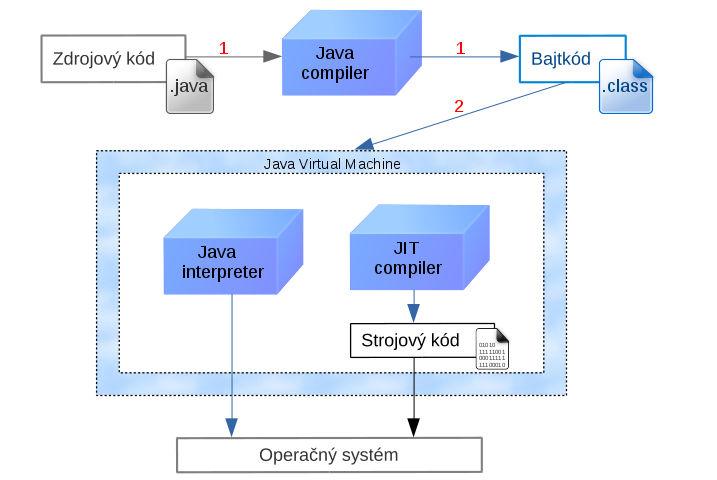
\includegraphics[width=0.96\textwidth]{JVM.png}
  \caption{Grafické znázornenie prekladu a spustenia programu, zdroj: vlastné
  spracovanie}
  \label{fig:jvm}
\end{figure}

Táto práca sa zaoberá popisom vlastností a implementáciou niekoľkých príkladov 
používajúcich nástroje na modifikáciu \textit{class} súborov. 
Konkrétne nástroje spomínané a používané v tejto práci sú \textit{Byteman} a
\textit{Javassist}.

Dokument sa skladá z dvoch logických celkov. Kapitoly dva až päť tvoria
teoretickú časť, ktorá popisuje bajtkód, \textit{Java Virtual Machine},
zavádzače tried, vlastnosti samotných nástrojov \textit{Byteman a Javassist}. 
Šiesta kapitola spomínané nástroje porovnáva.

Kapitola sedem sa venuje praktickým ukážkam, ktoré boli vytvorené vrámci
bakalárskej práce. Podkapitoly sa zaoberajú príkladmi, ktoré pokrývajú
oblasti detekcie volania výnimiek, detekcie nesprávne ošetrených výnimiek,
zlepšenia produkčného kódu a optimalizácie neefektívnych častí kódu. Každá z
ukážok demonštruje funkcionalitu jedného zo spomínaných nástrojov.

\chapter{Bajtkód}
\label{chap:bytecode}

Po preklade zdrojových kódov prekladačom \textit{javac} je každej
triede, prípadne rozhraniu programu, priradený jeden \textit{class} súbor,
popisujúci jej vlastnosti a funkcionalitu.

Pri načítaní \textit{class} súboru prijme JVM takzvaný prúd inštrukcií
bajtkódu (\textit{bytecode stream}) pre každú metódu triedy. V prípade volania
konkrétnej metódy za behu programu, sú inštrukcie danej metódy vykonávané.
Každá z nich je reprezentovaná číselnou hodnotou, nazývanou
\textit{opcode}. Zároveň má každá inštrukcia aj textovú podobu (\textit
{mnemonic}). V \textit{class} súboroch sú uložené v numerickej 
podobe.

Táto kapitola popisuje základný formát \textit{class} súboru a následne stručne
charakterizuje inštrukčnú sadu bajtkódu.~\footnote{Nasledujúci text vychádza 
zo 4. až 6. kapitoly špecifikácie JVM~\cite{Lindholm:2013:JVM:2462629}.}

\section{Štruktúra \textit{class} súboru}
\label{sec:classFile}
\textit{Class} súbor vždy pozostáva z jedinej štruktúry \textit{ClassFile}.
Táto štruktúra jednoznačne identifikuje konkrétnu triedu, 
prípadne rozhranie, definuje jej premenné a metódy.

Nasledujúci popis určuje sadu dátových typov použitých v texte. Typy
\textit{u1}, \textit{u2}, a \textit{u4} reprezentujú neznamienkové jedno, 
dvoj, alebo štvor-bajtové číslo. Pre znázornenie \textit{class} súboru je 
použitá pseudo-štruktúra v notácií jazyka C. Obsah štruktúry je popísaný ako 
zoznam po sebe nasledujúcich položiek.

\begin{example}{Formát \textit{ClassFile} štruktúry}
\begin{verbatim}
ClassFile {
  u4 magic;
  u2 minor_version;
  u2 major_version;
  u2 constant_pool_count;
  cp_info constant_pool[constant_pool_count-1];
  u2 access_flags;
  u2 this_class;
  u2 super_class;
  u2 interfaces_count;
  u2 interfaces[interfaces_count];
  u2 fields_count;
  field_info fields[fields_count];
  u2 methods_count;
  method_info methods[methods_count];
  u2 attributes_count;
  attribute_info attributes[attributes_count];
}
\end{verbatim}
\end{example}

Konštanta \textit{magic} identifikuje formát súboru \textit{class},
jej hodnota je vždy rovná \textit{0xCAFEBABE}.

Položky \textit{minor\_version} a \textit{major\_version}
určujú verziu \textit{class} súboru. Napríklad \textit{minor\_version} s
hodnotou \textit{m} a \textit{major\_version} s hodnotou \textit{M} indikujú
verziu s hodnotou \textit{M.m}.

Hodnota položky \textit{constant\_pool\_count} je rovná množstvu záznamov
v \textit{constant\_pool[]}, plus jeden.

Úložisko záznamov \textit{constant\_pool[]} (v podobe poľa štruktúr)
obsahuje rôzne dôležité konštanty: mená tried,  mená rozhraní, názvy 
premenných a iné. Každý záznam spomínaného poľa pozostáva zo značky
(\textit{tag}) a indexu (\textit{name\_index}). Značka určuje typ záznamu. 
Tabuľka všetkých značiek je uvedená v prílohe \ref{tab:tab1}. Pomocou 
unikátneho indexu je následne možné odkazovať sa na záznamy v ďalších častiach 
bajtkódu. Existuje niekoľko typov štruktúr~\footnote{Všetky štruktúry \textit{
constant\_pool[]} sú popísane v špecifikácií
JVM~\cite{Lindholm:2013:JVM:2462629}.}
reprezentujúcich rôzne druhy ich záznamov. Napríklad štruktúra
\textit{CONSTANT\_String\_info} reprezentuje objekty typu \textit{String}, 
zatiaľ čo ďalšie podobné štruktúry ako napríklad
\textit{CONSTANT\_Methodref\_info} a 
\textit{CONSTANT\_InterfaceMethodref\_info} reprezentujú metódy 
triedy, prípadne rozhrania.

Hodnota \textit{access\_flags} ukladá oprávnenia prístupu k
informáciám a vlastnosti tejto triedy pomocou
indikátorov. Napríklad nastavenie indikátora \textit{ACC\_INTERFACE} znamená,
že \textit{class} súbor popisuje rozhranie. Tabuľka indikátorov je uvedená v prílohe \ref{tab:tab2}.

Položka \textit{this\_class} obsahuje index položky poľa 
\textit{constant\_pool[]} odkazujúci na štruktúru
\textit{CONSTANT\_Class\_info}~\footnote{\textit{CONSTANT\_Class\_info} je 
štruktúra \textit{constant\_pool}, ktorá
udáva triedu, alebo rozhranie.}. Reprezentuje triedu, respektíve
rozhranie, definované týmto \textit{class} súborom.

Hodnotou \textit{super\_class} je taktiež index poľa \textit{constant\_pool[]}
odkazujúci na štruktúru typu \textit{CONSTANT\_Class\_info}. Reprezentuje
priamu nadtriedu triedy definovanej aktuálnym \textit{class} súborom. V 
prípade, že ide o súbor popisujúci rozhranie, index odkazuje na triedu
\textit{Object}. Trieda \textit{Object} má ako jediná hodnotu
\textit{super\_class} nulovú.

Počet prípadných rozhraní, ktoré daná trieda implementuje, vyjadruje položka
\textit{interface\_count}. V prípade rozhrania je táto položka rovná počtu
jeho priamych nadrozhraní.

Pole \textit{interfaces[]} obsahuje indexy \textit{constant\_pool[]},
odkazujúce na štruktúru typu \textit{CONSTANT\_Class\_info}. Zahŕňa indexy
všetkých rozhraní, ktoré sú implementované aktuálnou triedou, prípadne sú 
priamymi nadrozhraniami \textit{class} súboru.

Položka \textit{fields\_count} je rovná počtu premenných triedy a premenných
inštancií (\textit{fields}) \textit{class} súboru.

Štruktúry typu \textit{field\_info} sú združené v poli \textit{fields[]}. Toto
pole zahŕňa každú premennú triedy. Neobsahuje však zdedené atribúty. Podrobne 
sa štruktúrou \textit{field\_info} zaoberá kapitola \ref{sec:fields}.

Hodnota položky \textit{methods\_count} vyjadruje počet štruktúr
\textit{method\_info} v poli \textit{methods[]}.

Položka \textit{methods[]} je poľom štruktúr typu \textit{method\_info}. Každá
štruktúra \textit{method\_info} popisuje metódu aktuálnej triedy, respektíve
rozhrania. Zahŕňa konštruktory, metódy triedy a
metódy inštancií. Neobsahuje žiadne zdedené metódy. Štruktúru
\textit{method\_info} popisuje podkapitola \ref{sec:methods}.

Hodnota \textit{attributes\_count} je rovná počtu atribútov poľa
\textit{attributes[]} \textit{class} súboru.

Pole \textit{attributes[]} obsahuje štruktúry typu \textit{attribute\_info}.
Atribútmi štruktúry \textit{ClassFile} sú napríklad: \textit{SourceFile},
\textit{Deprecated}, \textit{InnerClasses} a iné. Atribút \textit{SourceFile} 
slúži na reprezentáciu mena \textit{class} súboru. Spomínané pole môže 
obsahovať maximálne jeden takýto atribút. Atribút
\textit{Deprecated} môže byť použitý v prípade, že bola daná trieda nahradená
(\textit{deprecated}). Pri jej volaní môže prekladač upozorniť 
užívateľa, že sa odkazuje na nahradenú triedu~\footnote{Rovnakým spôsobom je
možné atribút \textit{Deprecated} aplikovať aj na premenné a metódy.}. Vo
všeobecnosti sa štruktúre \textit{attribute\_info} venuje
podkapitola \ref{sec:attributes}.

\subsection{Reprezentácia dátových typov}
\label{sec:descriptors}
Dátové typy sú v \textit{class} súboroch reprezentované vo formáte reťazcov
s kódovaním \textit{UTF-8}. Delíme ich na:
\begin{itemize}
\item dátové typy premenných,
\begin{itemize}
\item primitívne dátové typy
\item referenčné dátové typy
\item polia
\end{itemize}
\item dátové typy metód.
\end{itemize}

Primitívnym dátovým typom (\textit{byte}, \textit{int}, \textit{boolean}, …) 
je priradený popis v podobe znaku (\textit{B}, \textit{I}, …). Napríklad 
premenná typu \textit{int} je reprezentovaná znakom: \textit{I}.

Referenčné dátové typy reprezentuje popis v tvare: \textit{L<classname>;}, kde 
\textit{classname} je meno triedy, alebo rozhrania daného referenčného
dátového typu. Premenná typu \textit{Object} je interpretovaná ako:
\textit{java/lang/Object;}. 

Identifikačný reťazec jednorozmerného poľa typu \textit{T} sa značí
\textit{[T}, pričom počet znakov \textit{[} je rovný dimenzii poľa. Napríklad
trojrozmerné pole typu double : \textit{double d[][][]} generuje reťazec:
\textit{[[[D}.

Reťazec dátového typu metódy sa skladá z reťazcov pre dátový typ parametrov,
ohraničených v zátvorkách \textit{(P*)} a reťazca pre dátový typ návratovej
hodnoty \textit{R}. Univerzálny tvar reťazca je potom:
\textit{(P*)R}.
V prípade hodnoty \textit{null} je reťazcom návratovej hodnoty znak
\textit{V}. Napríklad metódu \textit{boolean long pow (int n, int k)}
reprezentuje reťazec: \textit{(II)J}, v prípade metódy
\textit{Object method(byte b)} by šlo o reťazec:
\textit{(B)Ljava/lang/Object;}. Komplexný prehľad reprezentácie dátových typov
je uvedený v prílohe \ref{tab:tab3}.

\subsection{Premenné tried a inštancií}
\label{sec:fields}
Premenné tried inštancií (\textit{fields}) \textit{class} súboru sú v poli
\textit{fields[]} reprezentované pomocou štruktúry \textit{field\_info}.
Formát štruktúry \textit{field\_info} je nasledovný:

\begin{example}{Štruktúra \textit{field\_info}}
\begin{verbatim}
field_info {
  u2 access_flags;
  u2 name_index;
  u2 descriptor_index;
  u2 attributes_count;
  attribute_info attributes[attributes_count];
}
\end{verbatim}
\end{example}

Položka \textit{access\_flags} je indikátorom oprávnenia prístupu k danej
premennej. Mená všetkých indikátorov spolu s ich interpretáciou a hodnotou sú 
uvedené v prílohe \ref{tab:tab4}.
     
Dvojbajtová hodnota \textit{name\_index} je index \textit{constant\_pool[]},
reprezentujúci meno premennej.

Podobne ako \textit{name\_index}, aj \textit{descriptor\_index} je dvojbajtová
položka odkazujúca sa na štruktúru v \textit{constant\_pool}. Na rozdiel od
mena premennej však popisuje dátový typ premennej.

Položka \textit{attributes\_count} vyjadruje počet všetkých atribútov 
uložených v poli \textit{attributes[]}.

Pole \textit{attributes[]} môže obsahovať ľubovoľné množstvo atribútov
popisujúcich premennú. Štruktúra reprezentujúca atribút je daná všeobecným
predpisom \textit{attribute\_info}. Atribúty premenných musia byť
reprezentované jednou zo štruktúr \textit{ConstantValue}, \textit{Synthetic},
\textit{Signature}, \textit{Deprecated}, \textit{RuntimeVisibleAnnotations},
prípadne \textit{RuntimeInvisibleAnnotations}. Atribút s menom
\textit{ConstantValue} popisuje konštantné statické premenné.
\textit{Synthetic} je používaný u položiek, ktoré sa nevyskytujú v zdrojovom 
kóde. Podrobne sa štruktúrou \textit{attribute\_info} zaoberá
podkapitola~\ref{sec:attributes}.

\subsection{Metódy}
\label{sec:methods}
Každá metóda triedy, prípadne rozhrania, je v poli \textit{methods[]} uložená
pomocou štruktúry \textit{method\_info}. Táto štruktúra má
nasledujúci formát:

\begin{example}{Formát \textit{method\_info}}
\begin{verbatim}
method_info {
  u2 access_flags;
  u2 name_index;
  u2 descriptor_index;
  u2 attributes_count;
  attribute_info attributes[attributes_count];
}
\end{verbatim}
\end{example}

Indikátor \textit{access\_flags} zahŕňa nastavenia prístupových práv a
vlastností metódy. Tabuľka indikátorov \textit{access\_flags} štruktúry
\textit{method\_info} sa nachádza v prílohe \ref{tab:tab5}.

Položky \textit{name\_index} a \textit{descriptor\_index} sú podobne ako u
\textit{field\_info} indexmi do \textit{constant\_pool}. Tieto indexy
v \textit{constant\_pool} odkazujú na štruktúry charakterizujúce meno a dátový typ metódy. Reprezentáciu dátových typov popisuje
podkapitola~\ref{sec:descriptors}.

Hodnota položky \textit{attributes\_count} vyjadruje presný počet atribútov
v poli \textit{attributes[]}.

Pole \textit{attributes[]} obsahuje dodatočné atribúty danej metódy.
Jednotlivé položky poľa sú reprezentované elementárnym predpisom
\textit{attributes\_info}. Každá
z položiek je jednou zo štruktúr: \textit{Code}, \textit{Exceptions},
\textit{Synthetic},\textit{Signature}, \textit{Deprecated},
\textit{RuntimeVisibleAnnotations}, \textit{RuntimeInvisibleAnnotations},
\textit{RuntimeVisibleParameterAnnotations},
\textit{RuntimeInvisibleParameterAnnotations},
prípadne \textit{AnnotationDefault}.
Atribút \textit{Code} je jedným z najdôležitejších. Obsahuje inštrukcie
bajtkódu popisujúce fungovanie metódy. Okrem abstraktných a natívnych metód, musí každá z nich obsahovať práve jeden atribút typu
\textit{Code}. Atribút \textit{Exceptions} zahŕňa indexy výnimiek, ktoré
metóda volá. Bližším popisom základného formátu štruktúry \textit{attributes\_info} sa
zaoberá nasledujúca podkapitola.

\subsection{Atribúty}
\label{sec:attributes}
Pojem atribút tejto podkapitoly vyjadruje práve atribúty používané v poli
\textit{attributes[]} štruktúr \textit{field\_info}, \textit{method\_info} a
\textit{Code\_attributes}. Všeobecný predpis všetkých atribútov je vyjadrený
štruktúrou \textit{attribute\_info}. Existuje niekoľko základných
preddefinovaných atribútov: \textit{SourceFile}, \textit{ConstantValue},
\textit{Code}, \textit{Exceptions}, \textit{InnerClasses}, \textit{Synthetic},
\textit{LineNumberTable}, \textit{LocalVariableTable}, \textit{Deprecated} a
iné. Líšia sa funkcionalitou a využitím jednotlivými časťami \textit{class}
súboru. Všetky atribúty vychádzajú z už spomínaného všeobecného predpisu
\textit{attribute\_info}, ktorý má nasledujúci formát:

\begin{example}{Štruktúra \textit{attribute\_info}}
\begin{verbatim}
attribute_info {
  u2 attribute_name_index;
  u4 attribute_length;
  u1 info[attribute_lenght];
}
\end{verbatim}
\end{example}

Položka \textit{attributes\_name\_index} je indexom do \textit{constant\_pool},
odkazujúcim na meno atribútu. Štvorbajtová položka \textit{attribute\_length} 
je rovná hodnote vyjadrujúcej dĺžku následných informácií, ktoré sú uložené v 
štruktúre \textit{info[attribute\_length]}. Informácie sa líšia na základe 
odlišnej funkcionality a využitia jednotlivých atribútov.

\section{Inštrukcie JVM}
Po načítaní \textit{class} súboru sa JVM najskôr uistí, že je daný
súbor v správnom formáte popísanom v kapitole \ref{sec:classFile}. Tento 
proces sa nazýva kontrola formátu (\textit{format checking}). Prvé štyri bajty 
musia vždy obsahovať magickú konštantu \textit{magic}. Všetky rozoznané 
atribúty musia mať správnu dĺžku. \textit{Class} súbor nesmie byť skrátený, 
ani obsahovať nadbytočné bajty. Podobne úložisko \textit{constant\_pool} 
nesmie obsahovať žiadne nerozoznateľné informácie. 

Inštrukcie bajtkódu načítanej metódy sú uložené v poli \textit{code[]}
atribútu \textit{Code}, štruktúry \textit{method\_info} daného \textit{class}
súboru. Štruktúra \textit{Code\_attribute} reprezentujúca atribút \textit{Code}
musí spĺňať obmedzenia definované JVM. Tieto obmedzenia rozdeľujeme na dve
základné kategórie: 

\begin{itemize}
\item Statické obmedzenia: Stanovujú rozloženie inštrukcií v poli \textit{code}
a priradenie operandov jednotlivým inštrukciám. Niektorými z nich sú napríklad:

\begin{itemize}
\item prvá inštrukcia musí začínať na indexe 0,
\item pole \textit{code} nesmie byť prázdne.
\end{itemize}

\item Štrukturované obmedzenia: Špecifikujú vzťahy medzi inštrukciami JVM. Ide
o podmienky, ako napríklad:

\begin{itemize}
\item žiadna lokálna premenná nemôže byť volaná predtým, ako jej bola priradená
hodnota,
\item pred volaním (nestatickej) metódy, respektíve premennej, musí byť
inicializovaná inštancia triedy, ktorá ju obsahuje.
\end{itemize}

\end{itemize}

Prekladače jazyka Java generujú \textit{class} súbory, ktoré spĺňajú požiadavky
popísané v predchádzajúcom odseku. JVM však nemá žiadnu záruku, že
\textit{class} súbor, ktorý požaduje, bol generovaný prekladačom. Metódou
verifikácie~\footnote{Ďalšie príklady obmedzení a podrobný popis verifikácie
\textit{class} súborov je dostupný v špecifikácií
JVM~\cite{Lindholm:2013:JVM:2462629}} \textit{class} súboru môže JVM určiť, či
daný súbor pochádza z dôveryhodného zdroja.

\subsection{Dátové typy}
Dátové typy JVM delíme do troch základných
kategórií:

\begin{itemize}
\item Primitívne dátové typy: byte, short, int, long, boolean, float, double.
\item Referenčné dátové typy: pole, inštancia triedy, rozhranie.
\item Typ \textit{returnAddress}: používaný výhradne inštrukciami
\textit{jsr}, \textit{ret} a \textit{jsr\_w}.
\end{itemize}

Väčšina uvedených typov má veľkosť 32 bitov, typy \textit{long} a
\textit{double} sú však 64 bitové, preto zaberajú dva sloty v zásobníku.

\subsection{Architektúra a inštrukčná sada}
Architektúra JVM je založená na dátovej~štruktúre~zásobník~\footnote{Dátová
štruktúra zásobník (\textit{stack}) funguje na princípe FIFO (\textit{first in
first out}), kde posledný vložený prvok je prvým vybraným.}, ktorej základnými
operáciami sú \textit{push} - vloženie prvku do zásobníka a \textit{pop} - 
výber prvku z vrcholu zásobníka. JVM nemá registre na ukladanie hodnôt, preto 
musia byť pred použitím všetky uložené na zásobník.

Na nasledujúcom jednoduchom príklade sú popísané základné inštrukcie bajtkódu
pre prácu s premennými a konštantami.

\begin{example}{Metóda \textit{greaterThen} pred a po kompilácií}
\begin{verbatim}
public int greaterThen(int intOne, int intTwo) {
  if (intOne > intTwo) {
    return 0;
  } else {
    return 1;
  }
}

0: iload_1
1: iload_2
2: if_icmple  7
5: iconst_0
6: ireturn
7: iconst_1
8: ireturn
\end{verbatim}
\end{example}

Inštrukcie \textit{iload\_1} a \textit{iload\_2} pridajú do zásobníka operandov
(ďalej len zásobník) hodnoty lokálnych premenných na indexoch 1 a 2. V tomto 
prípade ide o parametre \textit{intOne} a \textit{intTwo}. 

\begin{figure}[h]
  \begin{minipage}{0.55\textwidth}
     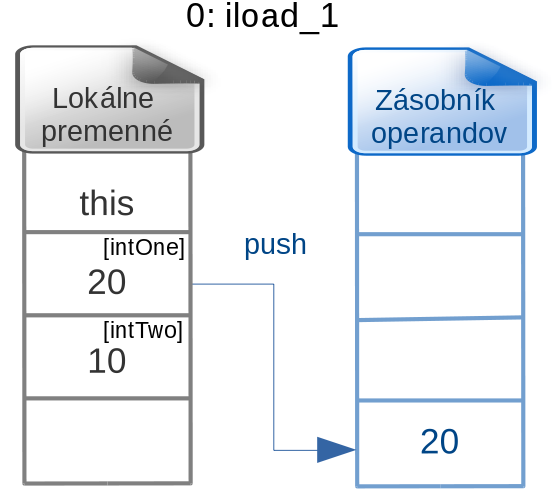
\includegraphics[width=0.825\textwidth]{iload_1.png}
  \end{minipage}
  \begin{minipage}{0.55\textwidth}
     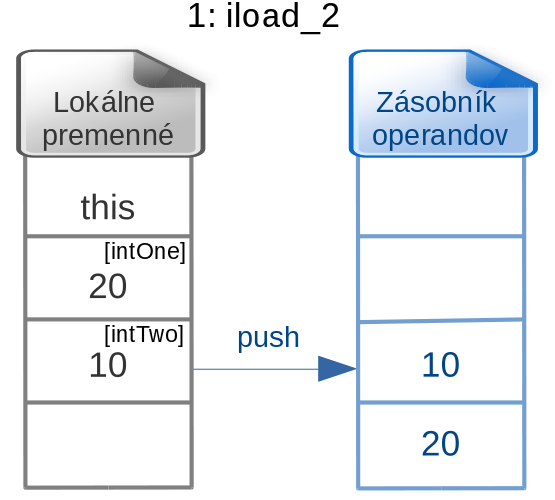
\includegraphics[width=0.825\textwidth]{iload_2.png}
  \end{minipage}
  \caption{Znázornenie funkcionality inštrukcií \textit{iload\_1} a
  \textit{iload\_2}, zdroj: vlastné spracovanie}
  \label{fig:gTiload}
\end{figure}

Vo všeobecnosti môžeme túto inštrukciu chápať ako \textit{xload} s predponou
\textit{x}, označujúcou primitívny dátový typ (napríklad: 
\textit{lload} pre long, \textit{fload} pre float). Existujú dva tvary, volania
tejto inštrukcie: 

\begin{itemize}
\item \textit{load\_<n>}, kde \textit{n} označuje index (celé číslo) lokálnej 
premennej, zároveň musí platiť: $0 \leq n \leq 4$,
\item \textit{load vindex}, kde pozíciou lokálnej premennej je hodnota
\textit{vindex}.
\end{itemize}

Ďalšou inštrukciou je \textit{if\_icmple} s parametrom 7, ktorá porovná dva 
objekty na vrchole zásobníka a prejde na siedmu inštrukciu v prípade, že je 
hodnota položky na vrchole zásobníka väčšia ako hodnota druhej položky. V 
príklade sú na zásobníku len položky, vložené predchádzajúcimi inštrukciami.
Podmienka teda platí v prípade, že hodnota parametra \textit{intOne} je menšia
než hodnota \textit{intTwo}. Vo všeobecnosti je možné podmienené výrazy 
vyjadriť pomocou inštrukcií: \textit{if\_acmp<cond>, if\_icmp<cond>, if<cond>,
ifnonnull, ifnull}.

Inštrukcie \textit{iconst\_0} a \textit{iconst\_1} vložia na zásobník hodnotu 
0, respektíve 1, v závislosti od vyhodnotenia podmienky \textit{if\_icmple}. 
Táto hodnota je následne vrátená inštrukciou \textit{ireturn}. Inštrukcie
\textit{iconst\_<n>, a ireturn} sú taktiež dostupné vo variantách s predponou 
ľubovoľného primitívneho dátového typu.

Dôkladný popis všetkých inštrukcií, vrátane ich parametrov, je uvedený v 
špecifikácií JVM~\cite{Lindholm:2013:JVM:2462629}.

\chapter{Zavádzače tried} 

Zavádzač je objekt zodpovedný za načítavanie tried. V JVM je reprezentovaný 
abstraktnou triedou \textit{ClassLoader}. Pomocou mena \textit{class} súboru by
mal zavádzač nájsť a generovať obsah, definujúci danú triedu. Každá
trieda obsahuje referenciu na konkrétny objekt typu \textit{ClassLoader}, 
ktorý ju definoval.~\cite{Oracle:ClassLoader}

Zvyčajne je trieda do JVM načítaná len v prípade, že je potrebná. Načítané sú 
zároveň všetky triedy, na ktoré sa odkazuje. Pomocou zavádzačov je
možné za behu programu dynamicky načítať ďalšie triedy, prípadne nové 
inštancie pôvodných tried.

Pri štandardnom načítaní triedy niektorá z implementácií triedy 
\textit{ClassLoader} vykoná nasledujúce tri kroky:
\begin{enumerate}
\item Skontroluje, či trieda už nebola načítaná.
\item Ak nebola, požiada nadtriedu o načítanie danej triedy. 
\item V prípade, že neuspeje, pokúsi sa načítať triedu pomocou
vlastného zavádzača.
\end{enumerate}

\subsection{Dynamické načítavanie tried}
K načítaniu novej triedy, napríklad \textit{MyClass}, do spusteného programu 
je potrebný objekt zavádzača. Získať ho je možné pomocou volania metódy 
\textit{MyClass.class.getClassLoader();}.
Novú triedu reprezentovanú súborom \textit{class} následne vráti metóda 
\textit{loadClass(class)} zavádzača.

\subsection{Znovunačítanie triedy}
Dynamické znovunačítanie triedy je mierne komplikovanejšie. Vstavané 
implementácie triedy \textit{ClassLoader} vždy kontrolujú, či trieda už nebola 
do JVM načítaná. Preto nie je možné žiadnu triedu načítať dvakrát pomocou 
vstavaných zavádzačov. Je nutné navrhnúť vlastnú implementáciu. Nasledujúci 
príklad znázorňuje formu implementácie vlastného zavádzača.

\begin{example}{Príklad zavádzača tried pre načítanie \textit{class} súborov zo
serveru}
\begin{verbatim}
     class NetworkClassLoader extends ClassLoader {
         String host;
         int port;

         public Class findClass(String name) {
             byte[] b = loadClassData(name);
             return defineClass(name, b, 0, b.length);
         }

         private byte[] loadClassData(String name) {
             // load the class data from the connection
              ...
         }
     }
\end{verbatim}
\cite{Oracle:ClassLoader}
\end{example}

Ďalšou komplikáciou je metóda \textit{ClassLoader.resolve()},
ktorá zabezpečuje linkovanie. Ide o metódu s atribútom \textit{final}, z čoho 
vyplýva, že ju nie je možné prepísať. Nepovolí však žiadnemu zavádzaču
linkovať dvakrát tú istú triedu. Preto je nutné pri každom ďalšom
znovunačítaní triedy vytvoriť jeho novú inštanciu.

\chapter{Byteman}
\label{chap:Byteman}

\textit{Byteman} je nástroj manipulujúci s bajtkódom, určený na modifikáciu 
Java aplikácií počas načítavania JVM, alebo za behu programu. 
Používa sa najmä na zjednodušenie trasovania a testovania aplikácií. Umožňuje 
používateľovi pridávať novú funkcionalitu do ktorejkoľvek časti programu.
Funguje bez nutnosti prepisovania a opätovnej kompilácie.

Modifikácia bajtkódu aplikácie je vykonávaná za behu programu. Preto je 
dovolená zmena Java kódu, popisujúceho časť tried JVM ako napríklad
\textit{String}, \textit{Thread} a podobne. Vďaka tejto funkcionalite je 
taktiež možné napríklad trasovanie správania sa JVM.

\textit{Byteman} používa jednoduchý jazyk
ECA~pravidiel~\footnote{ECA (\textit{event-condition-action}) pravidlá 
pozostávajú z udalosti, podmienky a akcie. Význam pravidla znamená: Ak nastane 
udalosť, skontroluj podmienku a v prípade, že platí, vykonaj
akciu~\cite{Sellis:ECARules}.} založený na Jave. Tieto ECA pravidlá
používa na špecifikáciu kde, kedy a ako má byť pôvodný Java kód transformovaný,
aby modifikoval danú triedu, prípadne rozhranie~\cite{RedHat:Byteman}.

\section{Byteman Agent}

Aby mohol \textit{Byteman} manipulovať s programom, musí mať tento program 
aktivovaný takzvaný \textit{Byteman Agent}, ktorý konfiguruje JVM pre prácu s 
pravidlami jeho jazyka.

Pri inštalácii agenta s prekladom programu je riešením použitie argumentu
nástroja \textit{java -javaagent}, ktorý zadáva cestu k \textit{JAR} súboru,
popisujúcemu pravidlá jazyka. Agentovi je možné pomocou argumentov
konfigurovať dve možnosti funkcionality:

\begin{itemize}
\item Základnou možnosťou je použiť argument \textit{script:[PATH]}, ktorý
načíta do programu skript definovaný pravidlami v súbore s cestou
\textit{PATH}.
\item V prípade potreby načítavania pravidiel do programu aj po spustení, je 
nutné nastaviť argument \textit{listener} na hodnotu \textit{true}. Do takto
spusteného programu je možné následne pomocou skriptu \textit{bmsubmit.sh}
pridávať a odoberať ľubovoľné pravidlá.
\end{itemize}

\textit{Byteman} je nastavený, aby neinjektoval kód tried JVM. Pri zmene tried
ako \textit{String a Thread} je preto nutné zmeniť túto vlastnosť
nastavením prepínača
[\textit{system property org.jboss.byteman.transform.all}]. Zároveň je
nutné zaistiť, aby bol \textit{Byteman Agent} načítaný (rovnako ako tieto 
triedy) defaultným (\textit{bootstrap}) zavádzačom.

Agenta je možné inštalovať taktiež do spustených aplikácií~\footnote{Typicky
ide o dlho bežiace aplikácie ako napríklad aplikačný server JBoss}, bez 
nutnosti ich opätovného spustenia. Slúži na to skript \textit{bminstall.sh}.
\textit{Byteman} je následne možné využiť ako nástroj na podrobnú kontrolu 
správania sa 
programu~\cite{RedHat:Byteman}. 

\section{Štruktúra jazyka pravidiel}
Pravidlá jazyka Byteman sú definované v skriptoch s príponou \textit{btm}.
Každé pravidlo pozostáva zo sekvencie definícií. Všeobecný predpis takto
definovaného pravidla je nasledovný:

\begin{example}{Kostra pravidla}
\begin{verbatim}
RULE <rule name>
CLASS <class name>
METHOD <method name>
BIND <bindings>
IF <condition>
DO <actions>
ENDRULE
\end{verbatim}
\end{example}

Definície musia byť zadané v správnom poradí, pričom prvou je vždy
\textit{RULE} a poslednou \textit{ENDRULE}. Základnými kategóriami pre
rozdelenie definícií pravidiel sú: Udalosti, Závislosti, Výrazy, Podmienky,
Akcie a iné. Všetky dôležité kategórie a definície sú popísané v nasledujúcich
sekciách kapitoly.

\subsection{Udalosti}
Udalosti pravidla (\textit{Rule Events}) identifikujú jeho umiestnenie v
metóde, nachádzajúcej sa v cieľovej triede.

Kľúčové slovo \textit{RULE}, nasledované menom pravidla, je ľubovoľným 
textovým reťazcom, pričom musí obsahovať medzeru. Kvôli rozlišovaniu 
jednotlivých pravidiel by mali byť tieto mená unikátne.

Rovnako definície \textit{CLASS} a \textit{METHOD} sú nasledované menami 
triedy a metódy, do ktorej bude pravidlo načítané. Meno triedy, prípadne 
rozhrania je možné špecifikovať aj bez cesty k balíku, v ktorom sa nachádza. V 
takomto prípade, Byteman spracováva každú triedu s daným menom, ktorá je do 
JVM načítaná. Definíciu \textit{CLASS} je možné nahradiť kľúčovým slovom
\textit{INTERFACE}, ktoré funguje rovnakým spôsobom ako \textit{CLASS}, no 
popisuje rozhranie. Doplnením znaku \^~na začiatok mena, je možné zabezpečiť 
dedičnosť, t.j. prenos pravidiel na potomkov.
Metódu je možné okrem samotného názvu špecifikovať aj jej návratovým typom, 
prípadne argumentami. Tieto bližšie špecifikácie nie sú povinné, preto je 
možné načítať pravidlo do viacerých preťažených metód zároveň.

Po nájdení metódy, respektíve metód, ktoré boli určené definíciami typu
\textit{CLASS}, \textit{METHOD}, prípadne \textit{INTERFACE}, je do každej z 
nich vložený spúšťač \textit{(triggerpoint)}. Tento spúšťač presne 
identifikuje miesto v metóde, kde bude bajtkód injektovaný. Pomocou 
špecifikácie je možné zvoliť rôzne pozície jeho umiestnenia v triede. 
Predvolenou hodnotou je \textit{AT ENTRY}, čo zaistí vloženie spúšťača na 
začiatok, teda pred prvú~inštrukciu~\footnote{Výnimkou sú inštrukcie volajúce 
konštruktor predka, prípadne alternatívny konštruktor.} danej metódy. Ďalšími 
možnosťami umiestnenia tohto spúšťača sú napríklad: \textit{AT EXIT},
\textit{AT LINE}, \textit{AT READ}, \textit{AT WRITE}. Tieto definície 
vkladajú spúšťač na koniec metódy, prípadne pred operáciu čítania, alebo 
zápisu do premennej. Tabuľka všetkých možností umiestnení sa nachádza v
prílohe \ref{tab:tab6}.

\subsection{Závislosti}
Skript definujúci  pravidlo jazyka \textit{Byteman} je možné obohatiť o 
závislosti pravidiel (\textit{Rule Bindings}). Tieto závislosti 
počítajú hodnoty niektorých premenných, ktoré môžu byť použité v ďalšom tele 
pravidla. Sú počítané pri každom spustení pravidla. Závislosti sú definované 
pomocou klauzule \textit{BIND}, nasledovanej názvom a prípadne typom premennej.
Každej premennej je pomocou výrazu nasledujúcim znamienko \qt{\textit{=}} 
priradená špecifická hodnota, napríklad:

\begin{example}{Závislosť}
\begin{verbatim}
RULE Bindings example
...
BIND thisClass = $0;
...
ENDRULE
\end{verbatim}
\end{example}

Vytvára premennú \textit{thisClass}, ktorej bude automaticky odvodený dátový typ a priraďuje jej hodnotu reprezentujúcu metódu tohto pravidla.

\subsection{Výrazy}
Výrazy (\textit{Rule expressions}) sa nachádzajú na pravej strane definície 
závislosti. Existujú dva základné typy výrazov:
\begin{itemize}
\item Jednoduché výrazy ako: referencie na predošlé závislosti, 
vstavané operátory (\textit{\$!, \$\^, \$@, …}), referencie na lokálne premenné v okolí spúšťača a mnohé iné.
\item Výrazy zložené z iných výrazov pomocou štandardných operátorov jazyka 
Java.
%operácie JVM.
\end{itemize}

Podmienkami pravidla (Rule Conditions) sú výrazy typu \textit{boolean}.
Tieto pravidlá nasledované klauzulu \textit{IF} sú overené po inicializácií závislostí.

\subsection{Akcie}
Jednou z najdôležitejších súčastí pravidla sú akcie pravidiel (\textit{Rule 
Actions}). Sú tvorené výrazmi, návratovými klauzulami, prípadne klauzulou
\textit{throw}. Na začiatku definície je klauzula \textit{DO}, ktorá je 
nasledovaná jednotlivými akciami. Každá akcia je na samostatnom riadku, 
oddeľuje ich bodkočiarka.

\begin{example}{Príklad použitia akcie}
\begin{verbatim}
RULE Actions example
...
DO System.out.println("This method is:" + $0);
   return;
...
ENDRULE
\end{verbatim}
\end{example}

Tento príklad znázorňuje zjednodušené pravidlo, ktorého akciou je výpis názvu 
metódy na štandardný výstup. 
%Narozdiel od ECA pravidiel nástroja \textit{Byteman}, Javassist používa na reprezentáciu \textit{class} súboru triedu \textit{Javassist.CtClass}.

\section{Použitie}
Primárne bol \textit{Byteman} určený na podporu testovania multivláknových a
multi-JVM aplikácií za použitia techniky nazývanej
\textit{Fault~Injection}~\footnote{V oblasti testovania softvéru tento pojem 
označuje techniku pre zlepšenie pokrytia testov vyvolaním chyby. Odstraňuje 
najmä chyby, ktoré by sa inak vyskytovali len
zriedka.~\cite{Roebuck:2011:STH:2031364}}. Zahŕňa preto 
funkcionalitu, ktorá bola navrhnutá na riešenie problémov súvisiacich s týmto 
typom testovania. \textit{Byteman} poskytuje podporu automatizácie v 
štyroch hlavných 
oblastiach:

\begin{itemize}
\item trasovanie špecifických väzieb kódu a zobrazovanie stavu danej
aplikácie, prípadne JVM,
\item narúšanie normálneho priebehu zmenou stavov, volanie neplánovaných
metód, vynucovanie návratových volaní, prípadne vyvolávanie neočakávaných 
výnimiek,
\item organizácia časovania aktivít vykonávaných nezávislými vláknami 
aplikácie,
\item monitorovanie a zhromažďovanie štatistík, pre sumarizáciu aplikácie a
operácií JVM.
\end{itemize}

V súčasnosti je \textit{Byteman} využívaný oveľa širšie pôvodný ako nástroj na
testovanie~\cite{RedHat:Byteman}. 

Najjednoduchším použitím \textit{Bytemana} je vkladanie kódu, ktorý trasuje 
správanie sa aplikácie. Zároveň môže byť využitý na monitorovanie,
alebo ladenie, ako aj na úpravu kódu pri testovaní a overenie správneho 
fungovania aplikácie. Pri vkladaní kódu na veľmi špecifické miesta je možné
vyhnúť sa režijným nákladom, ktoré často rastú pri ladení, alebo trasovaní 
produktu~\cite{Byteman:Homepage}.

\chapter{Javassist}

Ďalším nástrojom určeným na manipuláciu s bajtkódom je \textit{Javassist}. 
Tento nástroj využíva na manipuláciu s bajtkódom odlišný prístup ako
\textit{Byteman}. Narozdiel od ECA pravidiel, \textit{Javassist} používa na 
reprezentáciu \textit{class} súborov triedu \textit{Javassist.CtClass}.
Súbory je možné pomocou tejto triedy
modifikovať~\footnote{Možnosti modifikácie triedy pomocou \textit{CtClass} 
popisuje kapitola \ref{sec:mod}.} a následne modifikácie zapísať.

Na modifikáciu definície triedy je nutné najskôr získať referenciu na objekt
\textit{CtClass} z objektu \textit{ClassPool} pomocou jeho metódy
\textit{get()}.

\begin{example}{Získanie objektu \textit{CtClass}}
\begin{verbatim}
ClassPool pool = ClassPool.getDefault();
CtClass cc = pool.get("test.Rectangle");
\end{verbatim}
\end{example}

Vo vyššie uvedenom príklade je objekt typu \textit{CtClass}, ktorý reprezentuje
triedu \textit{test.Rectangle} vrátený objektom \textit{ClassPool} a uložený do
premennej \textit{cc}. Samotný objekt \textit{ClassPool} vrátila metóda 
\textit{getDefault}, ktorá prehľadáva defaultnú systémovú cestu. Z 
implementačného pohľadu je \textit{ClassPool} hešovacia tabuľka objektov
\textit{CtClass}, ktorá používa mená tried ako kľúče. Metóda \textit{get()} v
\textit{ClassPool} prehľadáva túto hešovaciu tabuľku, aby našla objekty typu
\textit{CtClass}, príslušné danému kľúču~\cite{Chiba:Javassist}.

Ďalšou možnosťou ovplyvňovania správania sa aplikácie je pridanie novo 
definovanej triedy. \textit{Javassist} túto funkcionalitu umožňuje pomocou 
metódy \textit{makeClass()}, volanej na objekte typu \textit{ClassPool}.

\begin{example}{Definícia novej triedy}
\begin{verbatim}
ClassPool pool = ClassPool.getDefault();
CtClass cc = pool.makeClass("Point");
\end{verbatim}
\end{example}

V tomto prípade je pomocou získaného kontajnera \textit{pool} definovaná nová 
trieda \textit{Point}. 

\section{Modifikácie}
\label{sec:mod}
Objekt \textit{CtClass} implementuje množstvo metód určených na modifikáciu triedy, 
ktorú reprezentuje. Výhodou použitia tohto nástroja spočíva aj v kompatibilite 
s rozhraním \textit{Java~Reflection}~\footnote{\textit{Java Reflection} je 
rozhranie bežne používané programami, ktoré vyžadujú schopnosť modifikácie 
správania sa spustenej Java aplikácie.~\cite{Oracle:JavaReflection}}.
\textit{CtClass} poskytuje metódy \textit{getName()}, \textit{getSuperClass()},
\textit{getMethods()} a mnohé iné. Taktiež obsahuje metódy pre úpravu definície
triedy. Povoľuje pridanie nového atribútu, konštruktora a metódy, prípadne 
modifikáciu tela existujúcej metódy~\cite{Chiba:Javassist}.

\subsection{Rozhranie pre prácu s bajtkódom}
Okrem štandardného rozhrania popísaného v predchádzajúcich odsekoch poskytuje 
\textit{Javassist} aj rozhranie pre priamu prácu s bajtkódom požadovanej 
triedy, respektíve metódy.

Rozhranie pracuje priamo s bajtkódom \textit{class} súboru. Napríklad metóda 
\textit{getClassFile()} triedy \textit{CtClass} vracia objekt typu 
\textit{ClassFile}, reprezentujúci daný súbor. Podobne metóda 
\textit{getMethodInfo()} triedy \textit{CtMethod} vracia objekt typu
\textit{MethodInfo}, predstavujúci štruktúru \textit{method\_info} daného 
\textit{class} súboru. Rozhranie používa notáciu JVM popísanú v kapitole 
\ref{chap:bytecode} a podrobne v
špecifikácii~JVM~\cite{Lindholm:2013:JVM:2462629}.

\section{Zápis do \textit{class} súboru}
Modifikácie vykonané v bajtkóde načítaných, prípadne novo vytvorených 
objektov, sa prejavia ihneď po zavolaní metódy \textit{writeFile()} triedy
\textit{CtClass}. Táto metóda preloží objekt \textit{CtClass} do \textit{class}
súboru, ktorý zapíše na disk. \textit{Javassist} taktiež poskytuje metódu 
\textit{toBytecode()}, ktorá vráti modifikované inštrukcie bajtkódu do poľa 
typu \textit{byte}~\cite{Chiba:Javassist}.

\chapter{Porovnanie}

Každý zo spomínaných nástrojov pristupuje k manipulácií s bajtkódom odlišným 
spôsobom. Zatiaľ čo \textit{Byteman} využíva jazyk ECA pravidiel, ktoré 
načítava pomocou takzvaného agenta, \textit{Javassist} je knižnicou jazyka 
Java. Táto kapitola oba nástroje stručne hodnotí a porovnáva:

\section{Vlastnosti nástroja \textit{Byteman}}
Výhodami použitia nástroja \textit{Byteman} sú:

\begin{itemize}
\item Prehľadnosť jazyka: Jazyk ECA pravidiel použitý nástrojom 
\textit{Javassist} je veľmi prehľadný a dobre zapamätateľný. 
\item Možnosť automatického generovania skriptov: Vďaka jednoznačnej štruktúre 
jazyka a jeho skriptov je možné pravidlá pomerne jednoducho generovať 
automaticky.
\end{itemize}

Na druhej strane má tento nástroj aj nevýhody. Najvýraznejšími z nich sú nasledujúce:

\begin{itemize}
\item Nutnosť manipulácie s vstavaným programom \textit{java agent} spustenej
aplikácie.
\item Obmedzená funkcionalita: Najväčšou nevýhodou nástroja 
\textit{Byteman} je nemožnosť editovania pôvodného kódu. \textit{Byteman} slúži
ako nástroj na pridávanie novej funkcionality, nijakým spôsobom však nedokáže 
editovať, prípadne odstrániť funkcionalitu pôvodnú. 
\end{itemize}

\section{Vlastnosti knižnice \textit{Javassist}}
Použitie knižnice \textit{Javassist} má nasledujúce 
výhody:

\begin{itemize}
\item Jednoduchá manipulácia: Keďže je \textit{Javassist} knižnicou jazyka 
Java, je manipulácia s ním pomerne nenáročná.
\item Dvojité aplikačné rozhranie: \textit{Javassist} poskytuje, na rozdiel od 
nástroja \textit{Byteman}, okrem základného aj nízkoúrovňové rozhranie pre 
priamu manipuláciu s bajtkódom.
\item Široké uplatnenie: Na rozdiel od nástroja \textit{Byteman}, funkcionalita
knižnice \textit{Javassist} poskytuje aj nástroje na úpravu existujúceho kódu.
\end{itemize}

Takisto tento nástroj má niekoľko slabých stránok, nie sú však výraznými prekážkami v následnej manipulácií s ním:

\begin{itemize}
\item Mohutnosť aplikácie: Pri jednoduchých úlohách by mohlo mať použitie 
knižnice \textit{Javassist} za následok značné časové oneskorenie.
\item Nemožnosť automatizácie: Vzhľadom na povahu tejto knižnice nie je možné 
automatické generovanie zdrojového kódu jazyka Java pre manipuláciu s 
bajtkódom.
\end{itemize}

\section{Zhrnutie}
Z vyššie uvedených vlastností nástrojov \textit{Byteman} a \textit{Javassist} 
vyplývajú možnosti ich využitia. Vo väčšine aplikácií pre manipuláciu s 
bajtkódom spôsobom, ktorý modifikuje pôvodnú funkcionalitu, je nutné použitie 
knižnice \textit{Javassist}. Pre úpravy programov, napríklad v prípade 
trasovania správania sa aplikácií, je vhodnou alternatívou nástroj 
\textit{Byteman}.

\chapter{Praktické ukážky}

Kľúčovou súčasťou bakalárskej práce sú praktické ukážky. Každý z príkladov je 
navrhnutý pre jeden z nástrojov \textit{Byteman}, respektíve 
\textit{Javassist}. Konkrétne demonštrujú základné možnosti jeho využitia pre 
vývoj a trasovanie programov v Jave. Ukážky pokrývajú štyri oblasti:

\begin{itemize}
\item detekcia volania výnimiek, 
\item detekcia nesprávneho ošetrenia výnimiek,
\item zlepšenie a sprehľadnenie produkčného kódu,
\item optimalizácia neefektívnych častí kódu.
\end{itemize}

Príklady obsahujú dve ukážky z oblasti detekcie volania a ošetrovania výnimiek 
a dve ukážky, zamerané na optimalizáciu a zlepšenie kódu. V praxi sa nástroje 
ako \textit{Byteman} a \textit{Javassist} využívajú najmä v aplikačných 
serveroch, prípadné iných projektoch, ktorých opätovná kompilácia by bola 
príliš časovo a technicky náročná. V ukážkach budem z praktických dôvodov 
využívať na testovanie ich funkcionality menšie programové celky a demonštračné
programy.

\section{Detekcia volania výnimiek}
Prvou z ukážok je detekcia volania výnimiek spusteného programu. Ide o detekciu
všetkých výnimiek, ktoré sú v požadovanej triede volané pomocou kľúčového slova
\textit{throw}. V bajtkóde je konštrukcia tohto kľúčového slova reprezentovaná 
inštrukciou \textit{athrow}, ktorá zavolá výnimku predtým pridanú na vrchol 
zásobníka a zároveň zásobník vyčistí.

\begin{figure}[H]
  \centering
   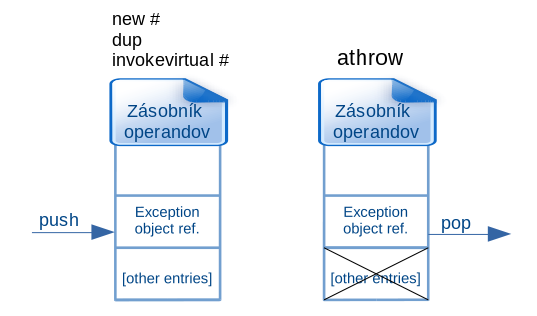
\includegraphics[width=0.80\textwidth]{throw.png}
  \caption{Grafické znázornenie pridania objektu výnimky a jej následné 
  vyvolanie pomocou inštrukcie \textit{athrow}, zdroj: vlastné spracovanie}
  \label{fig:throw}
\end{figure}

Detekcia volaných výnimiek je vhodným príkladom na ukážku využitia nástroja 
\textit{Byteman}. Ako bolo uvedené v kapitole \ref{chap:Byteman}, 
\textit{Byteman} využíva na popis modifikácie bajtkódu ECA pravidlá. 
Zovšeobecnené ECA pravidlá pre tento príklad sú v nasledujúcom tvare.

\begin{example}{Všeobecný formát ECA pravidla pre detekciu výnimiek metódy <m> 
volanej z triedy <C>}
\begin{verbatim}
RULE detect throw, method <m>, class <T>
  CLASS <T>
  METHOD <m>
  AT THROW ALL
  BIND exception:Throwable= $^
  IF true
  DO System.out.println("Detected athrow, exception: " + exception)
ENDRULE
\end{verbatim}
\end{example}

Klauzula \textit{RULE} udáva názov pravidla pre konkrétnu metódu a triedu. 
Nasledujú klauzuly \textit{CLASS} a \textit{METHOD}, ktoré špecifikujú ich 
názvy. V ďalšej časti pravidla sa nachádza jeho logika, ktorá popisuje 
zachytávanie výnimiek a reakciu na ich volanie v podobe výpisu na štandardný 
výstup.

Dôležitou súčasťou ukážkového programu je skript \textit{loadScripts.sh}, ktorý
tieto pravidlá generuje a načítava do už spustenej aplikácie~\footnote{Keďže 
skript pravidlá ihneď po vygenerovaní načítava, je nutné, aby už pred jeho 
spustením bežala aplikácia, ktorej výnimky bude sledovať. Táto aplikácia musí 
byť spustená s prepínačom \textit{agent listener}.}. Jediným 
potrebným argumentom je cesta ku \textit{class} súboru triedy, ktorej pravidlá 
bude skript generovať. Program následne monitoruje metódy zadanej triedy,
vrátane konštruktora. Taktiež je možné generovať a načítavať pravidlá
pre viacero tried zároveň. V tomto prípade je nutné zadať skriptu 
\textit{loadScripts.sh} cesty k ich \textit{class} súborom oddelené medzerou.

Po vygenerovaní a načítaní pravidiel program reaguje na každú volanú výnimku 
zadanej triedy, respektíve tried a pri detekcii na ňu upozorní. Pre účely tejto
práce používame ako demonštračný príklad aplikáciu s názvom 
\textit{fileChooser}~\footnote{Tento demonštračný príklad bol prevzatý z 
balíka Java Development Kit Demos and Samples.}. V reálnom prostredí by bolo 
možné detekciu volania výnimiek využiť napríklad v aplikačných serveroch, kde 
nie je volanie niektorých z nich vždy viditeľné.

\section{Detekcia nesprávneho ošetrenia výnimiek}
Nasledujúci príklad sa zaoberá detekciou nesprávne ošetrených výnimiek. V 
prípade zachytenia výnimky \textit{catch} blokom by mal program na túto 
situáciu vždy 
nejakým spôsobom reagovať (napríklad: logovaním udalosti, volaním inej výnimky,
riadeným pádom programu, …). Prázdne \textit{catch} bloky sú preto vo väčšine 
prípadov nesprávnym ošetrením danej výnimky.

Keďže ide o ukážku nástroja
\textit{Javassist} projektom je Java aplikácia vo formáte \textit{Maven}. 
Program postupne prechádza všetky metódy a konštruktory triedy, ktorú
monitoruje. Pri nájdení prázdneho \textit{catch} bloku uloží informácie o jeho
polohe do logu a na záver vypíše získané údaje.

\begin{example}{Výstup aplikácie po kontrole triedy example.tables.JDBCAdapter}
\begin{verbatim}
- Class JDBCAdapter -
Apr 28, 2015 6:15:18 PM application.CatchBlockTracer trace
INFO: -> Suspicious catch block found on line: 116 in method:
      example.tables.JDBCAdapter.executeQuery(java.lang.String)
Apr 28, 2015 6:15:18 PM application.CatchBlockTracer trace
INFO: -> Suspicious catch block found on line: 266 in method:
      example.tables.JDBCAdapter.setValueAt(java.lang.Object,…)
Apr 28, 2015 6:15:18 PM application.CatchBlockTracer trace
INFO: -> Suspicious catch block found on line: 81 in method:
      example.tables.JDBCAdapter(java.lang.String,…)
Apr 28, 2015 6:15:18 PM application.CatchBlockTracer trace
INFO: -> Suspicious catch block found on line: 79 in method:
      example.tables.JDBCAdapter(java.lang.String,…)
SUMMARY: 4 suspicious catch blocks found in class JDBCAdapter
\end{verbatim}
\end{example}

V tomto výstupe vidíme, že boli nájdené 4 nesprávne ošetrené výnimky na 
riadkoch: 79, 81, 166, 266.

\subsection{Štruktúra a funkčná logika aplikácie}
Aplikačnú logiku som rozdelil medzi nasledujúce štyri triedy balíka
\textit{application}: \textit{Tracer}, \textit{CatchBlockTracer},
\textit{CBDetector} a \textit{CBIndicesHandler}. 

Trieda \textit{Tracer} slúži na spustenie aplikácie pre ľubovoľnú 
triedu \textit{<C>}. Obsahuje metódu \textit{traceCatchBlocks(Class 
classToTrace)}, ktorej argumentom je objekt reprezentujúci \textit{<C>}. Táto 
metóda prevedie triedu na objekt \textit{CtClass} a následne z neho získa 
všetky metódy a konštruktory v podobe polí tried \textit{CtMethod} a 
\textit{CtConstructor}. Následne za pomoci triedy \textit{CatchBlockTracer} 
získa informácie o polohe všetkých prázdnych \textit{catch} blokov týchto 
metód a konštruktorov. 

Ako bolo uvedené v predchádzajúcom odseku, trieda \textit{CatchBlockTracer} je 
určená na spracovanie objektov \textit{CtMethod} a \textit{CtConstructor}. 
Hlavnou metódou triedy je \textit{trace(final CtBehavior cm)}. Metóda má jeden 
argument typu \textit{CtBehavior}, ktorého potomkami sú práve triedy
\textit{CtMethod} a
\textit{CtConstructor}. Uchováva si informácie o pozícií \textit{catch} blokov 
v podobe mapy, ktorej kľúčom je index prvej inštrukcie \textit{catch} bloku v 
bajtkóde a hodnotou je jeho pozícia v zdrojovom súbore. Túto mapu získava za 
pomoci tried \textit{CBDetector} a \textit{CBIndicesHandler}. Po získaní 
údajov o polohe všetkých blokov v danej metóde je každý z nich 
skontrolovaný metódou \textit{isEmpty}. V prípade preukázania nesprávne 
ošetrenej výnimky sú informácie \textit{catch} bloku uložené a logované. 

Mechanizmus kontroly prázdneho bloku prebieha pomocou nízkoúrovňového 
rozhrania knižnice \textit{Javassist} pre prácu s bajtkódom. V bajtkóde je 
každý \textit{catch} blok reprezentovaný vo forme znázornenej na obrázku 
\ref{fig:catch}.

\begin{figure}[h]
  \centering
   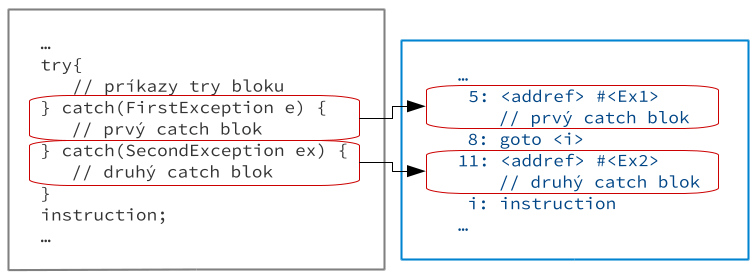
\includegraphics[width=\textwidth]{catch.png}
  \caption{Grafické znázornenie reprezentácie \textit{catch} bloku v bajtkóde,
  zdroj: vlastné spracovanie}
  \label{fig:catch}
\end{figure}

Na začiatku je na zásobník vložená referencia na objekt danej výnimky. 
Nasleduje telo \textit{catch} bloku. Premenná \textit{<i>} reprezentuje index 
inštrukcie vykonávanej bezprostredne po poslednom bloku. 
V prípade, že aktuálny \textit{catch} blok nie je posledným v 
rade, je za jeho telo vložená inštrukcia \textit{goto}, ktorá odkazuje na 
index inštrukcie \textit{<i>}. Metóda \textit{isEmpty} preto kontroluje, či 
telo bloku obsahuje iba inštrukciu skoku na index \textit{<i>}, 
prípadne či je úplne prázdne. 

Poslednými triedami na spodnej časti hierarchie v abstrakcii získavania polohy 
\textit{catch} blokov sú \textit{CBDetector} a \textit{CBIndicesHandler}. 
Slúžia na získanie mapy indexov \textit{catch} blokov pre zadanú metódu, 
prípadne konštruktor. Dôležitým nástrojom samotného vyhľadávania je metóda 
triedy
\textit{CtBehavior instrument(ExprEditor)}. Argumentom tejto metódy je práve 
objekt triedy \textit{CBIndicesHandler}.

\subsection{Testovacie príklady}
Okrem samotnej aplikácie projekt obsahuje aj dva balíky
\textit{example.simple} a \textit{example.tables}, na ktorých je možné 
funkcionalitu aplikácie testovať. Každý z balíkov obsahuje vlastnú spustiteľnú 
triedu \textit{Demo}, ktorá volá metódu 
\textit{application.Tracer.traceCatchBlocks} hlavnej aplikácie na jednotlivých 
testovacích triedach. 

Balík \textit{example.simple} obsahuje dve testovacie triedy, ktoré som 
vytvoril pre overenie funkčnosti aplikácie balíka \textit{application}. Po 
spustení aplikácia upozorní na nesprávne ošetrenie \textit{catch} blokov v 
triede \textit{PersonFactory}.

Balík \textit{example.tables} obsahuje komplexnejšie testovacie triedy, 
prevzaté z ukážok \textit{Java Development Kit Demos and Samples}. Výstupom 
spustenia triedy \textit{Demo} je kontrola tried \textit{JDBCAdapter}, \textit{
OldJTable} a \textit{TableExample}. Na nesprávne ošetrené výnimky sú tentokrát 
upozornené metódy a konštruktor triedy \textit{JDBCAdapter}.

Triedy testovacích balíkov je možné ľubovoľne modifikovať pre jednoduché 
testovanie funkcionality aplikácie. V prípade potreby testovania aplikácie na 
novej triede je nutné volať metódu hlavného balíka \textit{application
Tracer.traceCatchBlocks}
s argumentom špecifikujúcim danú triedu.

\section{Zlepšenie a sprehľadnenie produkčného kódu}
Program prispievajúci k zlepšeniu produkčného kódu sa špecializuje na náhradu 
priamych volaní atribútov generovanými \textit{get} a \textit{set} metódami. Vo
všeobecnosti aplikácia manipuluje s bajtkódom dvoch tried. Prvou z tried
je~\textit{<C1>}. Obsahuje atribúty, ku ktorým však neexistujú prístupové
\textit{get} a \textit{set} metódy, atribúty sú teda používané priamo. Trieda
\textit{<C2>} zapisuje a číta obsah týchto atribútov
\textit{<C1>}. Popísaná
implementácia porušuje základný princíp zapuzdrenia, ktorý by mal byť dodržaný 
za každých okolností. Projekt pod názvom \textit{code-improvement} preto slúži 
na generovanie prístupových metód k atribútom triedy \textit{<C1>} a následnú 
náhradu priamych volaní týmito metódami v triede \textit{<C2>}.

Aplikácia manipuluje s bajtkódom a \textit{class} súbormi požadovaných tried. 
Zmeny sa preto neprejavia v zdrojovom kóde. Rovnako by nemali nijako ovplyvniť 
vnútornú logiku modifikovaných tried. Okrem informácií zobrazených na 
štandardnom výstupe, je zmeny možné pozorovať aj v \textit{class} súboroch 
tried~\footnote{Class súbory je možné zobraziť v čitateľnej podobe napríklad 
prostredníctvom nástroja \textit{javap} príkazom \textit{[javap -c <path>]}.}.

\subsection{Štruktúra a funkčná logika aplikácie}
Aplikácia \textit{code-improvement} je projektom typu \textit{Maven}. 
Demonštruje využitie nástroja \textit{Javassist}. Projekt je tvorený dvoma 
balíkmi: \textit{application} a \textit{example}. Balík \textit{application} 
obsahuje samotný program nahradzujúci priame volania atribútov prístupovými 
metódami, ktorého základná funkcionalita bola načrtnutá v predchádzajúcich 
odsekoch. Balík \textit{example} je jednoduchým testovacím príkladom pre 
kontrolu funkčnosti tried balíka \textit{application}.

------------------------

TODO Diagram...

------------------------

Hlavným balíkom zabezpečujúcim fungovanie programu je \textit{application}. 
Funkcionalitu som tentokrát rozložil medzi 3 triedy: \textit{FieldChecker}, 
\textit{AccGenerator} a \textit{AccCreator}.

Trieda \textit{FieldChecker} je jedinou triedou, ktorá slúži na prístup k 
aplikácii. Po vytvorení objektu \textit{FieldChecker} pre triedy \textit{<C1>} 
a \textit{<C2>} dôjde volaním metódy \textit{FieldChecker.fixFieldsAccess()} k 
manipulácií s bajtkódom \textit{<C1>} a \textit{<C2>} spôsobom popísaním v 
prvom odseku tejto kapitoly. Metóda je preto len prístupovým bodom, ktorý 
využíva funkcionalitu ostatných metód a tried balíka \textit{application}.

Program postupne iteruje cez všetky atribúty triedy \textit{<C1>}. Pre každý 
z nich vytvorí \textit{AccGenerator} a následne \textit{AccCreator} prístupové
\textit{get} a \textit{set} metódy. Akonáhle sú tieto metódy úspešne načítané 
do bajtkódu \textit{<C1>}, vykoná metóda \textit{replaceFieldAccess()} náhradu 
priameho volania atribútu prístupovými metódami. Využíva k tomu najmä nástroj 
\textit{CodeConverter} knižnice \textit{Javassist}.

\textit{}

----------------------------------------

TODO Grafické znázornenie...

-----------------------------------------

Za generovanie a načítanie prístupových metód je zodpovedná trieda 
\textit{AccGenerator} a jej pomocná trieda \textit{AccCreator}. Táto pomocná 
trieda slúži na generovanie konkrétnych šablón prístupových metód pre zadaný 
atribút. Šablóny sa následne trieda \textit{AccGenerator} pokúsi načítať do
\textit{<C1>}.

\subsection{Testovací príklad}
Balík \textit{example} obsahuje jednoduchý príklad na otestovanie vyššie 
popísanej funkcionality. Spustiteľnou triedou daného príkladu je 
\textit{example.Demo}. Po jej spustení sa program pokúsi:

\begin{enumerate}
\item Vytvoriť a inicializovať triedu \textit{application.FieldChecker}.
\item Vykonať modifikáciu tried \textit{example.Initializer} a 
\textit{example.Triangle} (nedodržiavajú princíp zapuzdrenia) volaním metódy 
\textit{fixFieldsAccess()}.
\item Skontrolovať funkčnosť modifikovaných tried ich použitím.
\end{enumerate}

V prípade úspešnej modifikácie požadovaných tried by mal výstup vyzerať približne nasledovne:

\begin{example}{Výstup testovacieho príkladu pre aplikáciu
\textit{code-improvement}}
\begin{verbatim}
+ Getter for field: [a] in class [example.Triangle] was
  successfully created
+ Setter for field: [a] in class [example.Triangle] was
  successfully created
-> Read and write operations replaced for field
   [Triangle.a] in class [example.Initializer]

+ Getter for field: [b] in class [example.Triangle] was
  successfully created
+ Setter for field: [b] in class [example.Triangle] was
  successfully created
-> Read and write operations replaced for field
   [Triangle.b] in class [example.Initializer]

+ Getter for field: [c] in class [example.Triangle] was
  successfully created
+ Setter for field: [c] in class [example.Triangle] was
  successfully created
-> Read and write operations replaced for field
   [Triangle.c] in class [example.Initializer]

-------------------------------
Trying to use modified classes: 

Created: Circle {radius is 5.0Vertex centre: [0.0, 0.0]}
Created: Vertices of Triangle are {Vertex A: [-1.0, -1.0],
         Vertex B: [1.0, -1.0], Vertex C: [1.0, 1.0]}

Get and set methods successfully tested.
\end{verbatim}
\end{example}

Ak modifikácia neprebehla, napríklad v prípade opätovného spustenia na 
rovnakých triedach, vypíše program hlášku, ktorá upozorňuje užívateľa, že 
triedy, ktoré zadal, už boli v minulosti upravené.

Program je možné aplikovať na ľubovoľné triedy, následne definované v
 konštruktore
\textit{application.FieldChecker}~\footnote{V prípade, že ide o triedy mimo 
projektu \textit{code-improvement} je potrebné zadať do argumentu konštruktora 
aj cestu k balíku obsahujúcemu \textit{class} súbory triedy \textit{<C2>}.}.

\section{Optimalizácia neefektívnych častí kódu}
Posledný z príkladov sa zaoberá optimalizáciou neefektívne generovaných častí 
bajtkódu. Vo všeobecnosti vykonáva na bajtkóde mnoho optimalizácií JVM. 
Existuje však mnoho druhov ďalších úprav, pomocou ktorých je možné bajtkód 
výrazne zefektívniť.

Jednými z najčastejšie sa vyskytujúcich inštrukcií sú inštrukcie typu 
\textit{store} a \textit{load}. Ich úlohou je vkladanie, respektíve výber 
položiek zo zásobníka. Pri opakovanej modifikácií jednej premennej teda vzniká 
veľké množstvo nadbytočných operácií zápisu a čítania jej hodnoty. Vhodnou 
optimalizáciou je preto odstránenie nadbytočných inštrukcií.

Cieľom tohto programu je identifikovať a odstrániť nadbytočné inštrukcie 
čítania a zápisu v prípade aritmetických operácií na premenných typu 
\textit{double}. 

Keďže vyžaduje priamu prácu s bajtkódom a jeho modifikáciu, je táto 
optimalizácia vhodným príkladom pre demonštráciu funkcionality oboch rozhraní 
knižnice \textit{Javassist}.

\subsection{Štruktúra a funkčná logika aplikácie}
Triedy popisujúce logiku aplikácie sa opäť nachádzajú v balíku 
\textit{application}. Program sa skladá z troch tried: 
\textit{ArithmeticOptimizer}, \textit{MethodModifier} a 
\textit{InstructionVerifier}. Triedou pre prístup k programu je 
\textit{ArithmeticOptimizer}. Zvyšné triedy sú prístupné len v rámci balíka 
\textit{application}, mimo neho by nemali byť nijako používané.

Kľúčovou triedou programu je \textit{ArithmeticOptimizer} s prístupovou
metódou
\textit{optimizeClass(String classNameToOpt)}. Po jej inicializácií a spustení 
program iteruje cez všetky metódy triedy definovanej jediným argumentom 
\textit{classNameToOpt}. Každá metóda je následne optimalizovaná pomocou 
triedy \textit{MethodModifier}. Na záver je prepísaný \textit{class} súbor 
danej triedy a poskytnutá sumarizácie zmien.

Ako bolo uvedené vyššie, trieda \textit{MethodModifier} slúži na priamu 
optimalizáciu zadanej metódy. Daná metóda je reprezentovaná pomocou triedy 
\textit{MethodInfo}, ktorá knižnici \textit{Javassist} slúži ako popis 
rovnomenného atribútu \textit{class} súboru. Najdôležitejšou metódu triedy 
\textit{MethodModifier} je \textit{optimize()}. Táto metóda prechádza všetky 
inštrukcie bajtkódu a v prípade nájdeného nadbytočného páru \textit{dstore}, 
\textit{dload} tieto inštrukcie odstráni.

Program zvyčajne spracováva viac než jednu premennú pre danú metódu. Obrázok
\ref{fig:identify} popisuje kvôli prehľadnosti proces identifikácie
nadbytočných inštrukcií čítania a zápisu jednej premennej \textit{<n>}:

\begin{figure}[h]
  \centering
   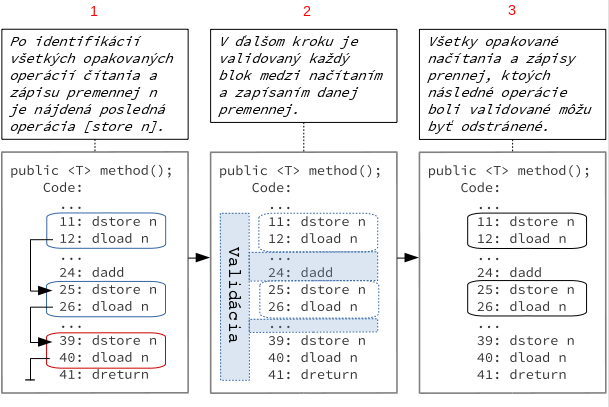
\includegraphics[width=\textwidth]{identification.png}
  \caption{Znázornenie identifikácie nadbytočných inštrukcií čítania a zápisu 
  premennej, zdroj: vlastné spracovanie}
  \label{fig:identify}
\end{figure}

Ako nástroj na identifikáciu typu aktuálnej inštrukcie slúži programu trieda 
\textit{InstructionVerifier}. Obsahuje metódy určujúce inštrukcie 
\textit{dstore} a \textit{dload}. Pomocou týchto metód je zároveň možné získať 
hodnotu argumentu spomínaných inštrukcií. Metóda \textit{isArithmetic(int op)} 
rozhoduje, či inštrukcia definovaná argumentom \textit{op} reprezentuje 
aritmetickú operáciu.

Balík \textit{example} obsahuje dva príklady, na ktorých je možné aplikáciu 
testovať. Každý z príkladov má spustiteľnú triedu \textit{Demo}, ktorá sa 
pokúsi optimalizovať vlastnú testovaciu triedu. Balík \textit{example.simple} 
optimalizuje jednoduchú triedu \textit{ArithmeticExample}, ktorá vykonáva 
aritmetické operácie. Balík \textit{example.model} je príklad podobný 
demonštračnému príkladu úlohy z predchádzajúcej kapitoly. Podrobné fungovanie 
testovacích príkladov je uvedené v \textit{Javadocu} a
komentároch~\footnote{Podrobnosti o uvedených príkladoch sú uvedené aj
v \textit{README} súbore projektu.}.

\begin{figure}[h]
  \centering
   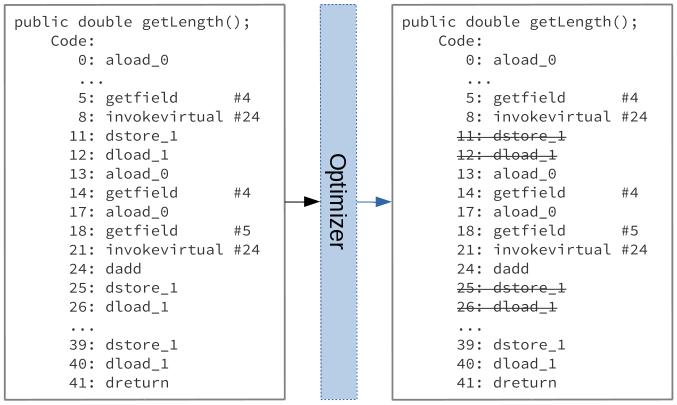
\includegraphics[width=\textwidth]{optimizer.png}
  \caption{Znázornenie optimalizácie bajtkódu jednej z metód balíka
  \textit{example.model}, zdroj: vlastné spracovanie}
  \label{fig:opt}
\end{figure}

Aplikáciu je takisto možné spustiť na ľubovoľnej triede vhodnej na 
optimalizáciu aritmetických operácií volaním metódy
\textit{application.Arithmetic Optimizer.optimizeClass(String classNameToOpt)}.

\chapter{Záver}

Hlavným cieľom práce bola analýza, porovnanie a implementácia sady príkladov
nástrojov určených na manipuláciu s bajtkódom jazyka Java. Nástrojmi použitými
v tejto práci boli \textit{Byteman} a \textit{Javassist}. 

Problematika manipulácie s bajtkódom má veľmi široké uplatnenie v mnohých
odvetviach vývoja a testovania softvéru. Demonštračné príklady boli preto
orientované na štyri vybrané oblasti:

\begin{itemize}
\item detekcia volania výnimiek,
\item detekcia nesprávneho ošetrenia výnimiek,
\item zlepšenie produkčného kódu,
\item optimalizácia neefektívnych častí kódu.
\end{itemize}

Analýzou vlastností spomínaných nástrojov vyplynuli možnosti ich funkcionality
a následné uplatnenie v príkladoch. 

Z vlastností nástroja \textit{Byteman} vyplýva, obmedzenie jeho použitia u
obmedzenej množiny aplikácií. Tento nástroj nie je možné využiť na 
editovanie pôvodného bajtkódu. Jeho funkcionalita je týmto obmedzená
na pridávanie vlastného kódu. Uplatnenie bolo možné v prípade
detekcie volania výnimiek spustenej aplikácie. Pri používaní sa nástroj javí
stabilný a veľmi dobre ovládateľný.

Knižnica \textit{Javassist} bola vďaka svojej rozsiahlej funkcionalite použitá
takmer vo všetkých príkladoch. Manipulácia s týmto nástrojom bola o niečo
náročnejšia. Výsledné príklady sú však badateľne využiteľnejšie. Najmä
programy v oblasti zlepšenia a optimalizácie kódu by bolo po rozpracovaní možné
použiť v praxi.

Vo väčšine projektov, ktoré manipulujú s bajtkódom je možné použiť knižnicu
\textit{Javassist}. Nástroj \textit{Byteman} je však vhodnou alternatívou najmä
v oblastiach trasovania a testovania programov.

\nocite{RedHat:Javassist}
\clearpage
\addcontentsline{toc}{chapter}{Literatúra} 
\bibliographystyle{alpha} 
\bibliography{bp} 

\appendix

\chapter{Tabuľky}

Zdrojom tabuliek 1 až 5 je špecifikácia
JVM~\cite{Lindholm:2013:JVM:2462629}.

\begin{table}
  \begin{tabular}{| l | c |}
    \hline
    \textbf{Constant Type} & \textbf{Value} \\
    \hhline{|=|=|}
    CONSTANT\_Class & 7 \\ \hline
    CONSTANT\_Fieldref & 9 \\ \hline
    CONSTANT\_Methodref & 10 \\ \hline
    CONSTANT\_InterfaceMethodref & 11 \\ \hline
    CONSTANT\_String & 8 \\ \hline
    CONSTANT\_Integer & 3 \\ \hline
    CONSTANT\_Float & 4 \\ \hline
    CONSTANT\_Long & 5 \\ \hline
    CONSTANT\_Double & 6 \\ \hline
    CONSTANT\_NameAndType & 12 \\ \hline
    CONSTANT\_Utf8 & 1 \\ \hline
    CONSTANT\_MethodHandle & 15 \\ \hline
    CONSTANT\_MethodType & 16 \\ \hline
    CONSTANT\_InvokeDynamic & 18 \\
    \hline
  \end{tabular}
  \caption{Tabuľka značiek určujúcich typ záznamu v \textit{constant\_pool}.
  Stĺpec \textit{Constant Type} označuje názov typu, stĺpec \textit{value}
  priraďuje každému typu číselnú hodnotu.}
  \label{tab:tab1}
\end{table}

\begin{table}
  \begin{tabular}{| l | c | p{6cm} |}
    \hline
    \textbf{Meno Indikátora} & \textbf{Hodnota} & \textbf{Interpretácia} \\
    \hhline{|=|=|=|}
    ACC\_PUBLIC & 0x0001 & Deklarovaná ako verejná; prístupná aj mimo balíka.
    \\ \hline
    ACC\_FINAL & 0x0010 & Deklarovaná ako final; žiadne podtriedy po 
    inicializácií. \\ \hline
    ACC\_SUPER & 0x0020 & Volá metódu nadtriedy, hlavne inštrukcia 
    invokespecial. \\ \hline
    ACC\_INTERFACE & 0x0200 & Je rozhranie, nie trieda.\\ \hline
    ACC\_ABSTRACT & 0x0400 & Deklarovaná ako abstraktná, nemôže byť 
    inštanciovaná. \\ \hline
    ACC\_SYNTHETIC & 0x1000 & Deklarovaná ako synthetic, nieje prítomná v 
    zdrojovom kóde. \\ \hline
    ACC\_ANNOTATION & 0x2000 & Deklarovaná ako typ annotation. \\ \hline
    ACC\_ENUM & 0x4000 & Deklarovaná ako typ enum. \\    
    \hline
  \end{tabular}
  \caption{Tabuľka indikátorov prístupových práv \textit{ClassFile} štruktúry.}
  \label{tab:tab2}
\end{table}

\begin{table}
  \begin{tabular}{| p{3cm} | c | p{6,5cm} |}
    \hline
    \textbf{Reprezentácia pomocou reťazca} & \textbf{Typ} & 
    \textbf{Interpretácia} \\
    \hhline{|=|=|=|}
     B & byte &  znamienkové celé číslo veľkosti jedného bajtu \\ \hline
     C & char & Znak s kódovaním UTF-16 \\ \hline
     D & double & číselná hodnota s dvojitou presnosťou a plávajúcou
     desatinnou čiarkou \\ \hline
     F & float & číselná hodnota s plávajúcou desatinnou čiarkou \\ \hline
     I & int & celé číslo \\ \hline
     J & long & celé číslo väčšieho rozsahu \\ \hline
     L ClassName ; & referencia & inštancia triedy ClassName \\ \hline
     S & short & znamienkové celé číslo krátkeho rozsahu \\ \hline
     Z & boolean & pravda alebo nepravda \\ \hline
     [ & reference & jednorozmerné pole \\
    \hline
  \end{tabular}
  \caption{Tabuľka reprezentácie dátových typov pre premenné.}
  \label{tab:tab3}
\end{table}

\begin{table}
  \begin{tabular}{| l | c | p{6,5cm} |}
    \hline
    \textbf{Meno Indikátora} & \textbf{Hodnota} & \textbf{Interpretácia} \\
    \hhline{|=|=|=|}
    ACC\_PUBLIC & 0x0001 & Deklarovaná ako verejná; prístupná aj mimo balíka.
    \\ \hline
    ACC\_PRIVATE & 0x0002 & Deklarovaná ako privátna; použiteľná len vrámci 
    triedy, v ktorej bola definovaná. \\ \hline
    ACC\_PROTECTED & 0x0004 & Deklarovaná ako protected; prístupná aj 
    podtriedam. \\ \hline
    ACC\_STATIC & 0x0008 & Deklarovaná ako statická. \\ \hline
    ACC\_FINAL & 0x0010 & Deklarovaná ako final; žiadne ďalšie priradenia po
    inicializácií. \\ \hline
    ACC\_VOLATILE & 0x0040 & Deklarovaná ako volatile; nemôže byť uložená do
    medzipamäte. \\ \hline
    ACC\_TRANSIENT & 0x0080 & Deklarovaná ako transient; nieje čítaná ani
    modifikovaná objektovým manažérom. \\ \hline
    ACC\_SYNTHETIC & 0x1000 & Deklarovaná ako synthetic, nieje prítomná v
    zdrojovom kóde. \\ \hline
    ACC\_ENUM & 0x4000 & Deklarovaná ako prvok objektu enum \\
    \hline
  \end{tabular}
  \caption{Tabuľka indikátorov prístupových práv a vlastností štruktúry
  \textit {field\_info}.}
  \label{tab:tab4}
\end{table}

\begin{table}
  \begin{tabular}{| l | c | p{5,5cm} |}
    \hline
    \textbf{Meno Indikátora} & \textbf{Hodnota} & \textbf{Interpretácia} \\
    \hhline{|=|=|=|}
    ACC\_PUBLIC & 0x0001 & Deklarovaná ako verejná; prístupná aj mimo balíka.
    \\ \hline
    ACC\_PRIVATE & 0x0002 & Deklarovaná ako privátna; použiteľná len vrámci 
    triedy, v ktorej bola definovaná. \\ \hline
    ACC\_PROTECTED & 0x0004 & Deklarovaná ako protected; prístupná aj 
    podtriedam. \\ \hline
    ACC\_STATIC & 0x0008 & Deklarovaná ako statická. \\ \hline
    ACC\_FINAL & 0x0010 & Deklarovaná ako final; nemôže byť prepísaná.
    \\ \hline
    ACC\_SYNCHRONIZED & 0x0020 & Deklarovaná ako synchronized; pri volaní je
    zabalená za použitia monitora. \\ \hline
    ACC\_BRIDGE & 0x0040 & Bridge metóda; je generovaná prekladačom. \\ \hline
    ACC\_VARARGS & 0x0080 & Deklarovaná s dynamickým počtom argumentov.
    \\ \hline
    ACC\_NATIVE & 0x0100 & Deklarovaná ako natívna; implementovaná v inom
    jazyku ako Java. \\ \hline
    ACC\_ABSTRACT & 0x0400 & Deklarovaná ako abstraktná, nieje implementovaná.
    \\ \hline
    ACC\_STRICKT & 0x0800 & Deklarovaná ako stricktfp, výpočty s plávajúcou
    čiarkou sú FP - strict. \\ \hline
    ACC\_SYNTHETIC & 0x1000 & Deklarovaná ako synthetic, nieje prítomná v
    zdrojovom kóde. \\
    \hline
  \end{tabular}
  \caption{Tabuľka indikátorov prístupových práv a vlastností štruktúry
  \textit {method\_info}.}
  \label{tab:tab5}
\end{table}

\begin{table}
  \begin{tabular}{| l | c |}
    \hline
    \textbf{Spúšťač} & \textbf{Argumenty} \\
    \hhline{|=|=|}
    AT ENTRY & - \\ \hline
    AT EXIT & - \\ \hline
    AT LINE & number \\ \hline
    AT READ & [type .] field [count | ALL ] \\ \hline
    AT READ & \$var-or-idx [count | ALL ] \\ \hline
    AFTER READ & [ type .] field [count | ALL ] \\ \hline
    AFTER READ & \$var-or-idx [count | ALL ] \\ \hline
    AT WRITE & [ type .] field [count | ALL ] \\ \hline
    AT WRITE & \$var-or-idx [count | ALL ] \\ \hline
    AFTER WRITE & [ type .] field [count | ALL ] \\ \hline
    AFTER WRITE & \$var-or-idx [count | ALL ] \\ \hline
    AT INVOKE & [ type .] method [ ( argtypes ) ] [count | ALL ] \\ \hline
    AFTER INVOKE & [ type .] method [ ( argtypes ) ][count | ALL ] \\ \hline
    AT SYNCHRONIZE & [count | ALL ] \\ \hline
    AFTER SYNCHRONIZE & [count | ALL ] \\ \hline
    AT THROW & [count | ALL ] \\
    \hline
  \end{tabular}
  \caption{Tabuľka možných umiestnení spúšťačov jazyka ECA pravidiel pre
  nástroj \textit{Byteman}.~\cite{RedHat:Byteman}}
  \label{tab:tab6}
\end{table}

\chapter{Obsah CD}
TODO - popis obsahu CD

%\begin{example}{Príklad implementácie vlastného \textit{class loaderu}.}
%\begin{verbatim}
%class NetworkClassLoader extends ClassLoader {
%  String host;
%  int port;
%
%  public Class findClass(String name) {
%    byte[] b = loadClassData(name);
%    return defineClass(name, b, 0, b.length);
%  }
%
%  private byte[] loadClassData(String name) {
%    // load the class data from the connection
%    …
%  }
%}
%\end{verbatim}
%\caption{Príklad zachytáva štruktúru vlastnej implementácie triedy
%\textit{ClassLoader}. \textit{NetworkClassLoader} by mohol slúžiť napríklad na
%načítanie dát zo siete. Zdroj: \cite{Oracle:ClassLoader}.}
%\label{ex:cLoader}
%\end{example}


\end{document}